\documentclass[tikz,border=2pt]{standalone}

% --- 定义颜色 ---
\definecolor{midBlue}{HTML}{1976D2}

\begin{document}
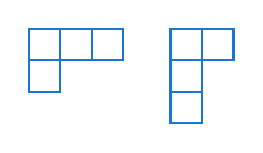
\begin{tikzpicture}[
    border_style/.style={thick}
]

    % --- 绘制宏 ---
    \newcommand{\yd}[4]{
        \node[inner sep=0] (#1) at (#2) {};
        \begin{scope}[shift={(#1.north west)}]
            \foreach \row [count=\r] in {#3} {
                \foreach \col in {1,...,\row} {
                    \draw[color=#4, border_style] (0.4*\col-0.4, -0.4*\r+0.4) rectangle ++(0.4, -0.4);
                }
            }
        \end{scope}
    }

    % --- 绘制图形 (紧凑排列) ---

    % 1. Partition [3,1] 放在原点
    \yd{p31}{0,0}{3,1}{midBlue}

    % 2. Partition [2,1,1] 放在右侧紧凑位置
    % [3,1]的最大宽度是 3*0.4 = 1.2cm。我们在 1.8cm 处放置下一个,间距为 0.6cm
    % 为了视觉平衡,稍微向下对齐一点 y=-0.2 (可选)
    \yd{p211}{1.8,0}{2,1,1}{midBlue}

\end{tikzpicture}
\end{document}